\documentclass[xcolor=x11names,compress]{beamer}

%% General document %%%%%%%%%%%%%%%%%%%%%%%%%%%%%%%%%%
\usepackage{graphicx}
\usepackage{tikz}
\usepackage{Tabbing}
\usetikzlibrary{decorations.fractals}
\usepackage{fancyvrb}
%%%%%%%%%%%%%%%%%%%%%%%%%%%%%%%%%%%%%%%%%%%%%%%%%%%%%%

%% Beamer Layout %%%%%%%%%%%%%%%%%%%%%%%%%%%%%%%%%%
\useoutertheme[subsection=false,shadow]{miniframes}
\useinnertheme{default}
\usefonttheme{serif}
\usepackage{palatino}
\usepackage{tabu}
% Links
\usepackage{hyperref}
\definecolor{links}{HTML}{003262}
\hypersetup{colorlinks,linkcolor=,urlcolor=links}

% addition of color
\usepackage{xcolor}
\definecolor{CoolBlack}{rgb}{0.0, 0.18, 0.39}
\definecolor{byellow}{rgb}{0.55037, 0.38821, 0.06142}
\definecolor{dgreen}{rgb}{0.,0.6,0.}
\definecolor{RawSienna}{cmyk}{0,0.72,1,0.45}
\definecolor{forestgreen(web)}{rgb}{0.13, 0.55, 0.13}
\definecolor{cardinal}{rgb}{0.77, 0.12, 0.23}

\setbeamerfont{title like}{shape=\scshape}
\setbeamerfont{frametitle}{shape=\scshape}

\setbeamercolor*{lower separation line head}{bg=CoolBlack}
\setbeamercolor*{normal text}{fg=black,bg=white}
\setbeamercolor*{alerted text}{fg=dgreen} % just testing; I think this looks better
\setbeamercolor*{example text}{fg=black}
\setbeamercolor*{structure}{fg=black}

\setbeamercolor*{palette tertiary}{fg=black,bg=black!10}
\setbeamercolor*{palette quaternary}{fg=black,bg=black!10}

% Margins
\usepackage{changepage}

\mode<presentation>
{
  \definecolor{berkeleyblue}{HTML}{003262}
  \definecolor{berkeleygold}{HTML}{FDB515}
  \usetheme{Boadilla}      % or try Darmstadt, Madrid, Warsaw, Boadilla...
  %\usecolortheme{dove} % or try albatross, beaver, crane, ...
  \setbeamercolor{structure}{fg=berkeleyblue,bg=berkeleygold}
  \setbeamercolor{palette primary}{bg=berkeleyblue,fg=white} % changed this
  \setbeamercolor{palette secondary}{fg=berkeleyblue,bg=berkeleygold} % changed this
  \setbeamercolor{palette tertiary}{bg=berkeleyblue,fg=white} % changed this
  \usefonttheme{structurebold}  % or try serif, structurebold, ...
  \useinnertheme{circles}
  \setbeamertemplate{navigation symbols}{}
  \setbeamertemplate{caption}[numbered]
  \usebackgroundtemplate{}
}

% Columns
\renewcommand{\(}{\begin{columns}}
\renewcommand{\)}{\end{columns}}
\newcommand{\<}[1]{\begin{column}{#1}}
\renewcommand{\>}{\end{column}}

\usepackage{cutwin}

% adding slide numbers
\addtobeamertemplate{navigation symbols}{}{%
    \usebeamerfont{footline}%
    \usebeamercolor[fg]{footline}%
    \hspace{1em}%
    \insertframenumber/\inserttotalframenumber
}

% equation stuff
\newcommand{\Macro}{\ensuremath{\Sigma}}
\newcommand{\Sn}{\ensuremath{S_N} }
\newcommand{\vOmega}{\ensuremath{\hat{\Omega}}}
\usepackage{mathrsfs}
\usepackage[mathcal]{euscript}
\usepackage{amssymb}
\usepackage{amsthm}
\usepackage{epsfig}
\usepackage{amsmath}
\newcommand{\ve}[1]{\ensuremath{\mathbf{#1}}}
\newcommand{\micro}{\ensuremath{\sigma}}
\newcommand{\detR}{\ensuremath{\Sigma}}

% title stuff for footer
\title{The PyNE Software Library}
\author{R.\ N.\ Slaybaugh}
\date{27 October 2014}

%%%%%%%%%%%%%%%%%%%%%%%%%%%%%%%%%%%%%%%%%%%%%%%%%%%%%%
\begin{document}



%%%%%%%%%%%%%%%%%%%%%%%%%%%%%%%%%%%%%%%%%%%%%%%%%%%%%%
%%%%%%%%%%%%%%%%%%%%%%%%%%%%%%%%%%%%%%%%%%%%%%%%%%%%%%
\begin{frame}
\title{The PyNE Software Library}
\subtitle{A Framework for ENSDF?}
\author{
\includegraphics[height=2cm]{../bk-eps-converted-to}\\R.\ N.\ Slaybaugh \\ Univ.\ of Cal.\ Berkeley}

\date{Nuclear Data Week\\ 6 November 2014\\ Brookhaven National Laboratory}
\titlepage
\end{frame}

%------------------------------------------------------
\begin{frame}{PyNE can be \underline{the} ENSDF processing tool}

	\begin{columns}
  	\begin{column}{0.45\textwidth}
 	   \begin{center}
 	   \begin{figure}
       \includegraphics[height=5cm]{../figs/pyne-icon-big}
       \caption{Python for Nuclear Engineering}
	   \end{figure}
 	   \end{center}
  	\end{column}
 	%
 	\begin{column}{0.45\textwidth}
 	   \begin{center}
 	   \begin{figure}
       \includegraphics[height=5cm]{../figs/person-with-tool}
       \caption{Can be \underline{the} tool for ENSDF processing}
	   \end{figure}
 	   \end{center}
  	\end{column}
	\end{columns}

\end{frame}

%------------------------------------------------------
\begin{frame}{Outline}

	\begin{columns}
  	\begin{column}{0.5\textwidth}
	    \begin{itemize}
          \item PyNE \cite{pyne}: what is it?
          \item PyNE as an ENSDF framework
          \item Other current initiatives
          \item Get involved!
	    \end{itemize}
  	\end{column}
 	%
 	\begin{column}{0.4\textwidth}
 	   \begin{center}
 	   \begin{figure}
       \includegraphics[height=4cm]{../figs/pyne-icon-big}
	   \end{figure}
 	   \end{center}
  	\end{column}
	\end{columns}

\end{frame}

%%%%%%%%%%%%%%%%%%%%%%%%%%%%%%%%%%%%%%%%%%%%%%%%%%%%%%
%%%%%%%%%%%%%%%%%%%%%%%%%%%%%%%%%%%%%%%%%%%%%%%%%%%%%%
\section{PyNE \cite{pyne}: what is it?}
\begin{frame}{What is PyNE?}

    PyNE is \textcolor{dgreen}{the} open source nuclear engineering toolkit.
    \vspace*{1em}
    \begin{itemize}
      \item PyNE is a \alert{library of composable tools} used to build
      nuclear science and engineering applications
      \item It is \alert{permissively licensed} (2-clause BSD)
      \item It supports both a \alert{c++} and a \alert{Python} API
      \item The name `PyNE' is a bit of a misnomer since most of the code
      base is in c++ but most daily usage happens in Python
      \item \alert{v0.4} is the current, stable release
      \item As an organization, PyNE was born in April 2011
      (however, core parts of PyNE have existed since 2007)
    \end{itemize}

\end{frame}

%------------------------------------------------------
\begin{frame}{What can PyNE do?}

    The idea is to be able to easily combine components and avoid redeveloping
    utilities someone else has developed.

    \begin{itemize}
      \item \alert{Nuclear data} and cross-section reading/processing
      \item Material handling
      \item Canonical nuclide and reaction naming conventions
      \item Mesh operations
      \item MCNP and Serpent input/output parsing
      \item Fuel cycle functionality (transmutation, enrichment)
      \item There's more, and the list continues to grow
    \end{itemize}

\end{frame}

%%%%%%%%%%%%%%%%%%%%%%%%%%%%%%%%%%%%%%%%%%%%%%%%%%%%%%
%%%%%%%%%%%%%%%%%%%%%%%%%%%%%%%%%%%%%%%%%%%%%%%%%%%%%%
\section{PyNE as an ENSDF framework}
%------------------------------------------------------
\begin{frame}{Nuclear Data in PyNE}

    PyNE already has some nuclear data support:
    \vspace*{1 em}
    \begin{itemize}
      \item ENSDF \alert{level} and \alert{decay} data
      \begin{itemize}
        \item parser
        \item conversion to hdf5
        \item access in c++ and Python
      \end{itemize}
      \item European Activation File cross sections
      \item Atomic mass data (KAERI)
      \item ENDF format cross section reader
      \item ACE format cross section reader
    \end{itemize}
\end{frame}

%------------------------------------------------------
\begin{frame}{Nuclear Data in PyNE}

	\begin{columns}[T]
  	\begin{column}{0.45\textwidth}
  	    \begin{center}
  	    \textbf{Structure Data}
  	    \end{center}
        \begin{itemize}
          \item 177 471 entries from IAEA ENSDF data
          \item Spin, parity, energy level
          \item Half-life, decay type, branching ratio
        \end{itemize}
  	\end{column}
 	%
 	\begin{column}{0.45\textwidth}
        \begin{center}
  	    \textbf{Decay Data}
  	    \end{center}
        \begin{itemize}
          \item Energy, intensity, initial, and final levels for:
          \begin{itemize}
            \item 116 598 gamma lines
            \item 13 230 electron capture/beta +
            \item 11 788 betas
            \item 2 552 alphas
          \end{itemize}
          \item 3868 unique primary decays
        \end{itemize}
  	\end{column}
	\end{columns}

    \vspace*{1 em}
    Let's look at a \alert{quick example}!

\end{frame}
%------------------------------------------------------

\begin{frame}{Consistency in ENSDF N and PN records}
    \begin{itemize}
        \item N record has photon intensity normalization (NR) and branching ratio (BR)
        \item PN record has entry for NRxBR
        \item ENSDF manual "recommends" NRxBR
        \item NRxBR is not always consistent (or meaningful)
        \item Consistency not checked with current tools
        \item 18 records contained significant inconsistencies
        \begin{itemize}
            \item NRxBR = 1 or NRxBR = 0 or mismatch $>$ 1\%
            \item including $^{241}$ Pu $\alpha$-decay
        \end{itemize}
        \item This issue was reported and fixed
        % Full list
        % 27NA    28NE B-N DECAY                2006TR02                  11NDS    2011
        % 29MG    31NA B-2N DECAY               1993KL02                  12NDS    2012
        % 48CR    49FE B+P DECAY                1996FA09                  06NDS    2006
        % 97Y     97Y IT DECAY (142 MS)         1996LH03,1996LH05,1986LH0110NDS    2010
        %105IN    105SN EC DECAY (34 S)         1995PF01                  05NDS    2005
        %110PD    110AG EC DECAY (24.56 S)      1965FR01                  12NDS    2012
        %110AG    110AG IT DECAY (249.83 D)     1965GE01,1993KA37,1975CL0312NDS    2012
        %110XE    114BA A DECAY (0.43 S)        2002MA19,1997JA12         12NDS    2012
        %111PD    111PD IT DECAY (5.5 H)        1977KR14                  09NDS    2009
        %111AG    111PD B- DECAY (5.5 H)        1977KR14,1969BE11,1969SC1209NDS    2009
        %111CD    111AG B- DECAY (64.8 S)       1977KR14                  09NDS    2009
        %114CD    114IN EC DECAY (49.51 D)      1969CO04                  12NDS    2012
        %139CS    252CF SF DECAY: ?             1974CLZX,1972HO08         01NDS    2001
        %154SM    154EU EC DECAY                1968ME12,2004TE01         09NDS    2009
        %192OS    192OS IT DECAY (5.9 S)        1970HEZH,1973PA21,1979KAYT12NDS    2012
        %197AU    197PT B- DECAY (19.8915 H)                              05NDS    2005
        %237U     241PU A DECAY                 1976GUZN,1968AH01,1965BA2606NDS    2006
        %254FM    254ES B- DECAY (39.3 H)       1973AH04                  05NDS    2005
    \end{itemize}

\end{frame}

\begin{frame}{Consistency in ENSDF N and PN records ....}
    %This "changes in the last month" snapshot includes most of the records above
    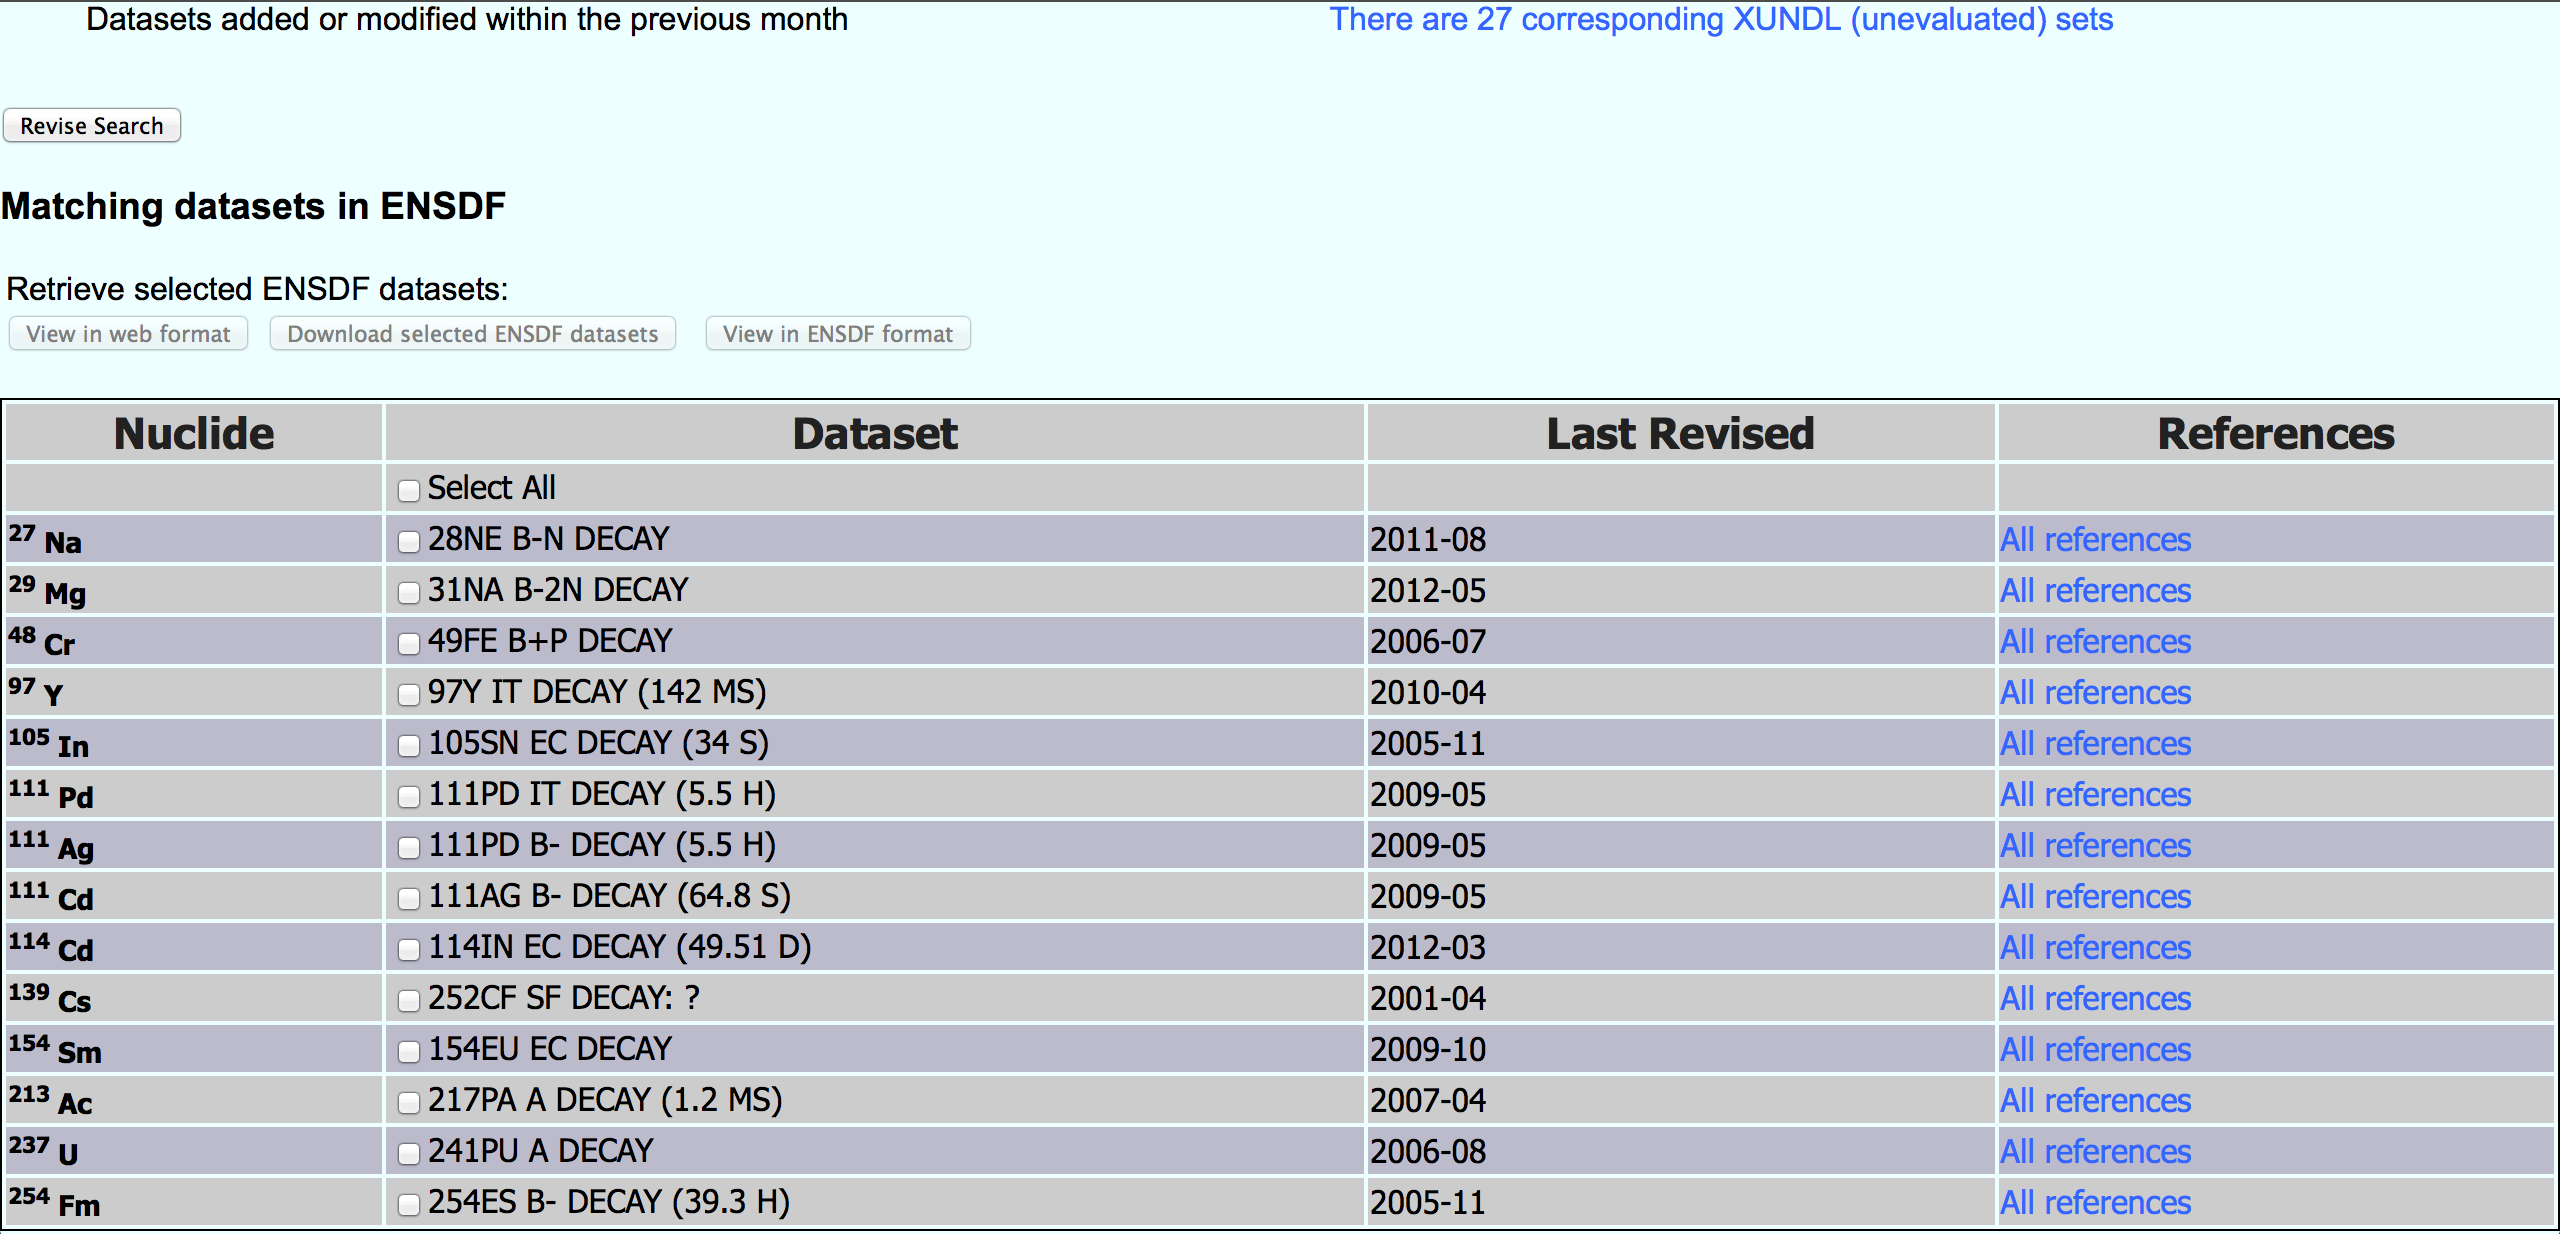
\includegraphics[height=5.5cm]{ensdf_updates}
\end{frame}
%------------------------------------------------------
\begin{frame}{Expanding into an ENSDF framework}

    Three iniatives:
    \begin{enumerate}
      \item Add handling of ENSDF \alert{reaction} data
       
      \item Wrap ENSDF \alert{Analysis} and(?) \alert{Utility} programs
      \begin{itemize}
        \item NSDFLIB
        \item ALPHAD, BrIcc, DELTA, GABS, GTOL, HSICC, LOGFT, PANDORA,
        RadList, RULER
        \item ADDGAM, Avetools, Visual Averaging Library, ENSDAT and 
        ComTrans, FMTCK, TREND (or replace through Python)
      \end{itemize}
        
      \item Add comparison utilities (based on \alert{community input})
    \end{enumerate}
    
\end{frame}

%%%%%%%%%%%%%%%%%%%%%%%%%%%%%%%%%%%%%%%%%%%%%%%%%%%%%%
%%%%%%%%%%%%%%%%%%%%%%%%%%%%%%%%%%%%%%%%%%%%%%%%%%%%%%
\section{Other current initiatives}
\begin{frame}{What else is happening in PyNE?}

    The biggest push: \alert{V\&V} $\rightarrow$ methodically making PyNE compliant
    with the QA standards we've ratified, which are based on the ASME NQA-1 standards
    \cite{pyne_vnv}

    \vspace*{1 em}
    Many other items (large and small) in our ``ticket" list

    \begin{center}
 	\begin{figure}
 	\includegraphics[height=1.75in,clip]{../figs/PyNE-tickets}
    \end{figure}
 	\end{center}

\end{frame}

%------------------------------------------------------
\begin{frame}{Verification and Validation}

    \textbf{Verification}: Have we built the software correctly?\\
    \textbf{Validation}: Have we built the correct software?

    \vspace*{1 em}
    Strategies employed by PyNE:

    \begin{itemize}
      \item Version control
      \item Formal review process
      \item Documentation: theory manual, user's guide, developer's guide, API,
      ticket system
      \item Test suite
      \item Continuous Integration
    \end{itemize}

\end{frame}

%------------------------------------------------------
\begin{frame}{GND and Fudge Support?}

    We have an open \href{https://github.com/pyne/pyne/issues/236}{ticket}
    for working with \alert{Fudge} to: 

    \vspace*{1 em}

    \begin{itemize}
      \item Create a cross section data source for GND backed by Fudge
      \item Create an ENDF data source backed by Fudge
      \item Investigate their processing routines
      \item Have a GND viewer (if Fudge doesn't)
    \end{itemize}
    
    The Fudge interface should happen after their next release\\
    \hspace*{1.5 em}(waiting on licensing issues)

\end{frame}

%%%%%%%%%%%%%%%%%%%%%%%%%%%%%%%%%%%%%%%%%%%%%%%%%%%%%%
%%%%%%%%%%%%%%%%%%%%%%%%%%%%%%%%%%%%%%%%%%%%%%%%%%%%%%
\section{Get involved!}
\begin{frame}{Why Would I Get Involved?}

    \begin{block}{As a \alert{user}:}
    \begin{itemize}
      \item You could do your work or research with PyNE
      \item You get the rest of PyNE's functionality
      \item You can take advantage of the assurance of the V\&V 
      about maintenance!
    \end{itemize}
    \end{block}

    \vspace*{1 em}
    \begin{block}{As a \alert{developer}:}
    \begin{itemize}
      \item You should be selfish
      \item Contribute to PyNE in ways that support the work that you are doing
      \item If a feature you want is not in PyNE right now, chances are that other
      people want to see that feature too
      \item This will help your future self as much as future other people
    \end{itemize}
\end{block}

\end{frame}

%------------------------------------------------------
\begin{frame}{How Can I Get Involved?}

    \begin{block}{Contact PyNE}
    \begin{itemize}
      \item Website: \href{http://pyne.io/}{\texttt{http://pyne.io/}}

      \item User's Mailing List: \href{pyne-users@googlegroups.com}
      {\texttt{pyne-users@googlegroups.com}}

      \item Developer's List: \href{pyne-dev@googlegroups.com}
      {\texttt{pyne-dev@googlegroups.com}}

      \item GitHub: \href{https://github.com/pyne/pyne}
      {\texttt{https://github.com/pyne/pyne}}

      \item Tutorial: \href{http://pyne.io/tutorial/index.html}
      {\texttt{http://pyne.io/tutorial/index.html}}
    \end{itemize}
    \end{block}

    \vspace*{2 em}
    \begin{block}{What goes into PyNE?}
    Anything that is not export controllable, proprietary,
    or under HIPPA restrictions!  (If you have questions, \emph{ask})
    \end{block}

\end{frame}


%%%%%%%%%%%%%%%%%%%%%%%%%%%%%%%%%%%%%%%%%%%%%%%%%%%%%%
%%%%%%%%%%%%%%%%%%%%%%%%%%%%%%%%%%%%%%%%%%%%%%%%%%%%%%
\section*{}
\begin{frame}[fragile]{Questions?}

    \begin{center}
    \includegraphics[height=3in,clip]{../questions-comic}
    \end{center}

\end{frame}

% --------------------------------------------------------------
\begin{frame}[fragile]{PyNE In the Literature}

    \begin{itemize}
      \item Intro: ``PyNE: Python For Nuclear Engineering'' \cite{pyne_intro}
      \item Progress reports: \cite{scopatz_pyne}, \cite{pyne_progress}
      \item In research: \cite{Biondo2014}, \cite{MarquezDamian2014280},
      \cite{Scopatz2013a}
      \item V\&V: ``Quality Assurance within the PyNE Open Source \\Toolkit''
      \cite{pyne_vnv}
      \item Poster at SciPy: \cite{scipy}
    \end{itemize}

\end{frame}
% --------------------------------------------------------------
\begin{frame}[allowframebreaks]{References}
	\bibliographystyle{unsrt}
	\bibliography{2014-PyNEforData}
\end{frame}

\end{document}
